
% Preamble
\documentclass[11pt]{report}

% Packages
\usepackage{amsmath}
\usepackage{graphicx}
\usepackage{color}
\usepackage[table,xcdraw]{xcolor}
\usepackage{multirow}

\usepackage[margin=2.5cm]{geometry}



% set image file paths
%\graphicspath{ {../../fuzzy/output/mamdani\_bell\_v9/io\_graphs/} }


\title{Funky Systems and Neural Networks}
\author{Jéssica Consciência e Tiago Leite}


\begin{document}
\maketitle
\newpage

\part{Fuzzy System}

%% Texto ainda por melhorar!!
Firstly we started by deciding between which type of fuzzy system
we should implement: Mamdani, Takagi-Sugeno or Tsukamoto. From the
project statement we observe that the output \textit{CLPVariation}
is not any clear function of the input, rulling out Takagi-Sugeno,
also meaning that our output is a \textbf{Fuzzy Set}. If we wish for
our output to be monotonic then the choice would be Tsukomoto, since
we did not want this restriction and decided for starting with a simple
approach then later on adding difficulty when needed.
(Early on we decided to try to make data-driven decisions with an iterative
improving process)

\section{First Iterations}

In the initial iteration, we selected the variables \textit{ProcessorLoad}, \textit{MemoryUsage}, and \textit{Latency} based on common sense.
These variables were chosen as inputs, while \textit{CLP} was designated as the output.
We opted for triangular membership functions, defining four levels for each input variable: (low, medium, high, critical) for \textit{ProcessorLoad} and \textit{MemoryUsage}, and (poor, fair, good, great) for \textit{Latency}.

To start building the system, we decided to focus on just two variables: \textit{MemoryUsage} and \textit{ProcessorLoad}.
We then defined the range of the membership functions associated with each term of the two linguistic variables.
Considering that a device with more than 85\% processor load or memory usage is typically unable to perform its basic tasks,
it became clear that this threshold would correspond to a specific term, which we labeled as ``critical''. The ranges for the other membership function terms were distributed between 0 and 1 based on what we deemed appropriate.
We also decided to keep the terms associated with \textit{CLP} straightforward, using only three terms: ``decrease'', ``increase'', and ``maintain''.
The values for the membership functions of these terms were distributed between -1 and 1.

The figures below illustrate the membership function graphs for these variables.

\begin{figure}[htbp]
    \centering
    \begin{minipage}{0.32\textwidth}
        \centering
        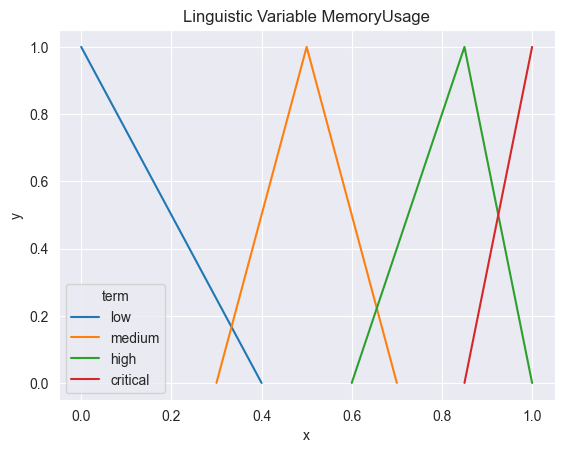
\includegraphics[width=\textwidth]{../images/triangular_MemoryUsage}
        \caption{Memory Usage}
        \label{fig:processor_load}
    \end{minipage}
    \hfill
    \begin{minipage}{0.32\textwidth}
        \centering
        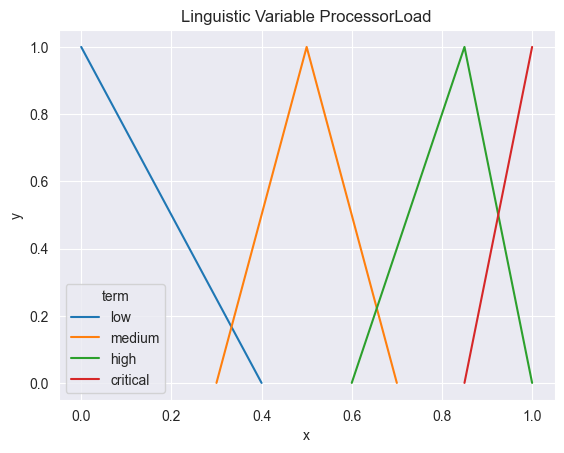
\includegraphics[width=\textwidth]{../images/triangular_ProcessorLoad}
        \caption{Processor Load}
        \label{fig:memory_usage}
    \end{minipage}
    \hfill
    \begin{minipage}{0.32\textwidth}
        \centering
        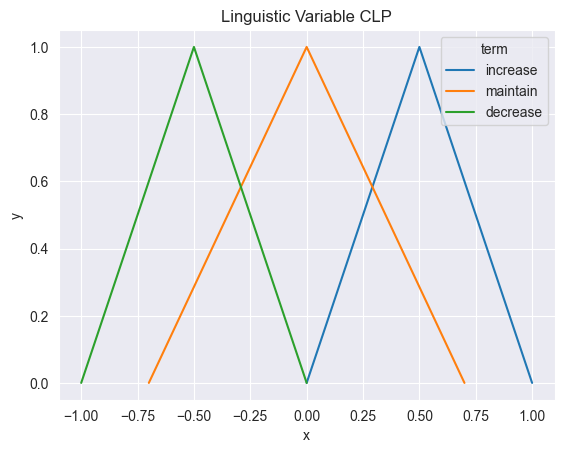
\includegraphics[width=\textwidth]{../images/triangular_CLP}
        \caption{CLP Variation}
        \label{fig:clp}
    \end{minipage}
\end{figure}



To visualize the system's output, we generated 50 data points for \textit{MemoryUsage} and \textit{ProcessorLoad} ranging between 0 and 1.
We then created an interactive 3D graph that showed the evolution of \textit{CLP} based on these two values.




Subsequently, we explored the effect of switching the membership functions to a Gaussian distribution.

\begin{figure}[h]
\centering
%\includegraphics{path_to_gaussian_graph}
%\caption{3D visualization of Gaussian membership functions}
\end{figure}

During the experimentation phase with different membership functions,the need for visualization became apparent.
To facilitate this, we developed a helper script [fuzzy/visualization/fuzzy\_system\_to\_dataframe] that converts the
FuzzySystem Python object into a dynamic dataframe, enabling easy plotting and analysis of the membership functions.



\section{Generalized Bell}
We decided to experiment with a more generic Membership function, so we
extended simpful's Base Membership Function class and created Bell\_MF [in fuzzy/models/bell\_mf.py].
The first results are shown in the figure bellow.

%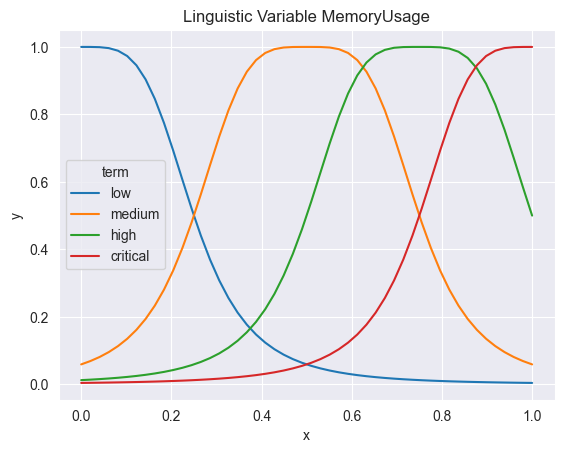
\includegraphics[width=0.5]{../../fuzzy/output/mamdani_bell/io_graphs/MemoryUsage.png}
%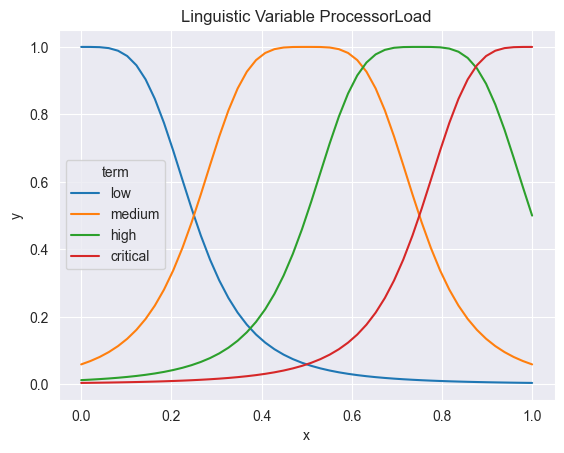
\includegraphics[width=0.5]{../../fuzzy/output/mamdani_bell/io_graphs/ProcessorLoad.png}
%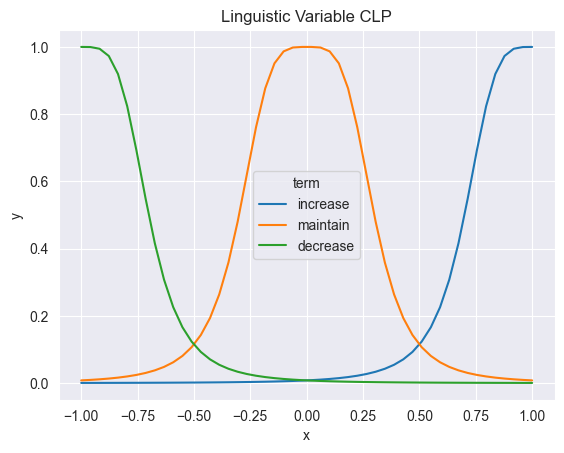
\includegraphics[width=0.5]{../../fuzzy/output/mamdani_bell/io_graphs/CLP.png}

%%
\section{Architecture}
This should contain choice of architecture and why.

\section{Membership Functions}
all the membership functions and linguistic terms

\begin{figure}

%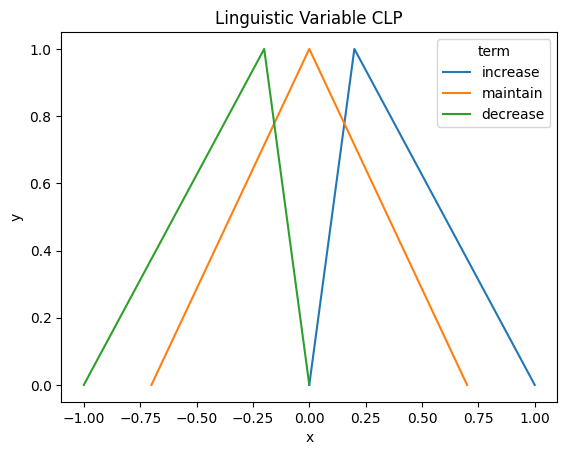
\includegraphics{CLP.png}
%\begin{tabular}[ccc]
%    \subfloat[caption]{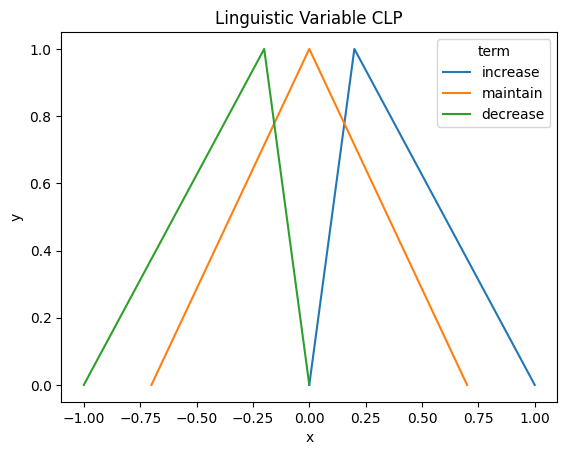
\includegraphics[width=.3\textwidth]{CLP.png}} & % noqa
%    \subfloat[caption]{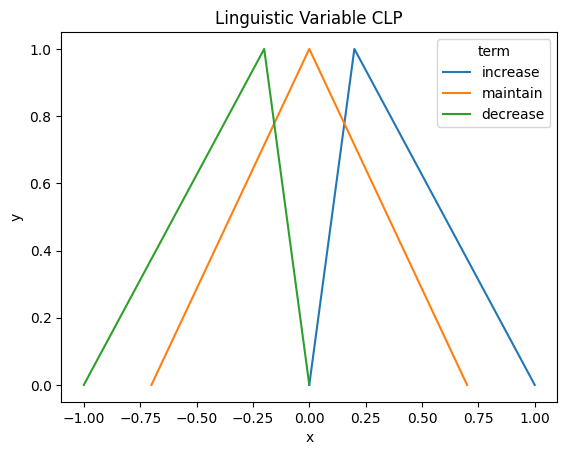
\includegraphics[width=.3\textwidth]{CLP.png}} &
%    \subfloat[caption]{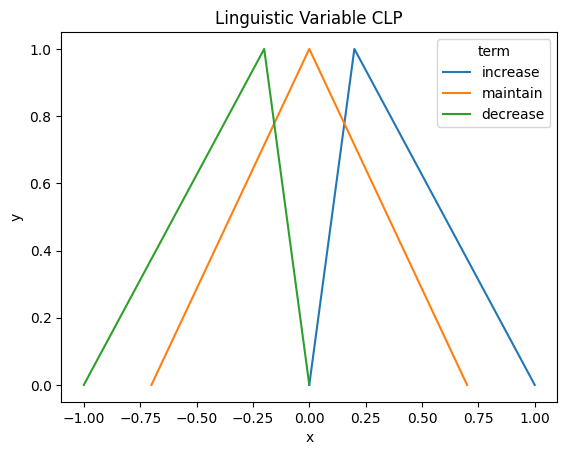
\includegraphics[width=.3\textwidth]{CLP.png}} \\
%\end{tabular}
\end{figure}

\section{Rules}
rules

\begin{table}
\begin{tabular}{|
>{\columncolor[HTML]{9698ED}}c l|cccc|}
\hline
\multicolumn{2}{|c|}{\cellcolor[HTML]{FFCC67}{\color[HTML]{333333} }}                                & \multicolumn{4}{c|}{\cellcolor[HTML]{9698ED}Latency}                                                        \\ \cline{3-6}
\multicolumn{2}{|c|}{\multirow{-2}{*}{\cellcolor[HTML]{FFCC67}{\color[HTML]{333333} CLP Variation}}} & \multicolumn{1}{l|}{low} & \multicolumn{1}{l|}{moderate} & \multicolumn{1}{l|}{high} & \multicolumn{1}{l|}{very high} \\ \hline
\multicolumn{1}{|c|}{\cellcolor[HTML]{9698ED}}                                     & low             & \multicolumn{1}{c|}{IS}  & \multicolumn{1}{c|}{IS}       & \multicolumn{1}{c|}{I}    & I                              \\ \cline{2-6}
\multicolumn{1}{|c|}{\cellcolor[HTML]{9698ED}}                                     & moderate        & \multicolumn{1}{c|}{I}   & \multicolumn{1}{c|}{I}        & \multicolumn{1}{c|}{I}    & I                              \\ \cline{2-6}
\multicolumn{1}{|c|}{\cellcolor[HTML]{9698ED}}                                     & high            & \multicolumn{1}{c|}{M}   & \multicolumn{1}{c|}{M}        & \multicolumn{1}{c|}{D}    & D                              \\ \cline{2-6}
\multicolumn{1}{|c|}{\multirow{-4}{*}{\cellcolor[HTML]{9698ED}System Load}}        & critical        & \multicolumn{1}{c|}{DS}  & \multicolumn{1}{c|}{DS}       & \multicolumn{1}{c|}{DS}   & DS                             \\ \hline
\end{tabular}
\end{table}


\section{Results}


\part{Neural Networks}



\end{document}
